\documentclass[11pt]{article}
\usepackage{latexsym}
\usepackage{amsmath}
\usepackage{amssymb}
\usepackage{amsthm}
\usepackage{epsfig}
\usepackage[tight]{subfigure}
\usepackage{xcolor}
\usepackage{amsmath}
\usepackage{mathtools}

\DeclareMathOperator*{\minimize}{min}
\DeclareMathOperator*{\maximize}{max}

\usepackage{algorithm}
 %on linux you may need to run sudo apt-get install texlive-full to install algorithm.sys
\usepackage{algorithmic}

\usepackage{verbatim}

\usepackage[breaklinks=true,bookmarks=false]{hyperref}
\hypersetup{
    colorlinks=true,
    linkcolor=red,
    filecolor=magenta,      
    urlcolor=blue,
}

\newcommand{\handout}[5]{
  \noindent
  \begin{center}
  \framebox{
    \vbox{
      \hbox to 5.78in { {#1} \hfill #2 }
      \vspace{4mm}
      \hbox to 5.78in { {\Large \hfill #5  \hfill} }
      \vspace{2mm}
      \hbox to 5.78in { {\em #3 \hfill #4} }
    }
  }
  \end{center}
  \vspace*{4mm}
}

\newcommand{\lecture}[5]{\handout{#1}{#2}{#3}{#4}{#5}}
\newcommand{\collision}[0]{\mathrm{collision}}
\newcommand{\nocollision}[0]{\overline{\collision}}

\newcommand*{\QED}{\hfill\ensuremath{\square}}

\newtheorem{theorem}{Theorem}
\newtheorem{corollary}[theorem]{Corollary}
\newtheorem{lemma}[theorem]{Lemma}
\newtheorem{observation}[theorem]{Observation}
\newtheorem{proposition}[theorem]{Proposition}
\newtheorem{definition}[theorem]{Definition}
\newtheorem{claim}[theorem]{Claim}
\newtheorem{fact}[theorem]{Fact}
\newtheorem{assumption}[theorem]{Assumption}
\newtheorem{note}[theorem]{Note}

\newcommand{\indep}{\perp \!\!\! \perp}

% 1-inch margins, from fullpage.sty by H.Partl, Version 2, Dec. 15, 1988.
\topmargin 0pt
\advance \topmargin by -\headheight
\advance \topmargin by -\headsep
\textheight 8.9in
\oddsidemargin 0pt
\evensidemargin \oddsidemargin
\marginparwidth 0.5in
\textwidth 6.5in

\parindent 0in
\parskip 1.5ex
%\renewcommand{\baselinestretch}{1.25}
% \newtheorem{theorem}{Theorem}

\begin{document}

\lecture{Statistical Techniques in Robotics (16-831, S21)}{Lecture \#02
  (Wednesday, February 3)}{Lecturer: Kris Kitani}{Scribes: Akshay Dharmavaram, Zongyue Zhao}{Online Learning (PWEA, Greedy)}

\section{Review}

\subsection{Introduction}

In the last lecture, we briefly went over the course logistics, then broke down the problem of robot learning along three axes: (1) whether the learner is exposed to all possible situations (exhaustive vs. sampled); (2) whether the learner receives feedback for all possible actions (instructive vs. evaluative); (3) whether the outcome of the current action affects the next action (sequential vs. one-shot) \cite{littman2015reinforcement}. In this lecture, we first introduced the concept of online learning, then briefly discussed Prediction with Expert Advice (PWEA). We also analyzed the theoretical upper bound of the number of mistakes a greedy PWEA learner could make, under the assumption of realizability.

\subsection{Robot Learning Problems}

Robotic systems are used in various situations. Before diving into the specific techniques best used in each situation, we need to characterize the robot learning problem \cite{connell_robot_2012}. As demonstrated in Figure \ref{fig:learning_prob}, we differentiate robot learning problems with the characteristics of feedback the learner receives from the environment. 

\begin{figure}[ht]
    \centering
    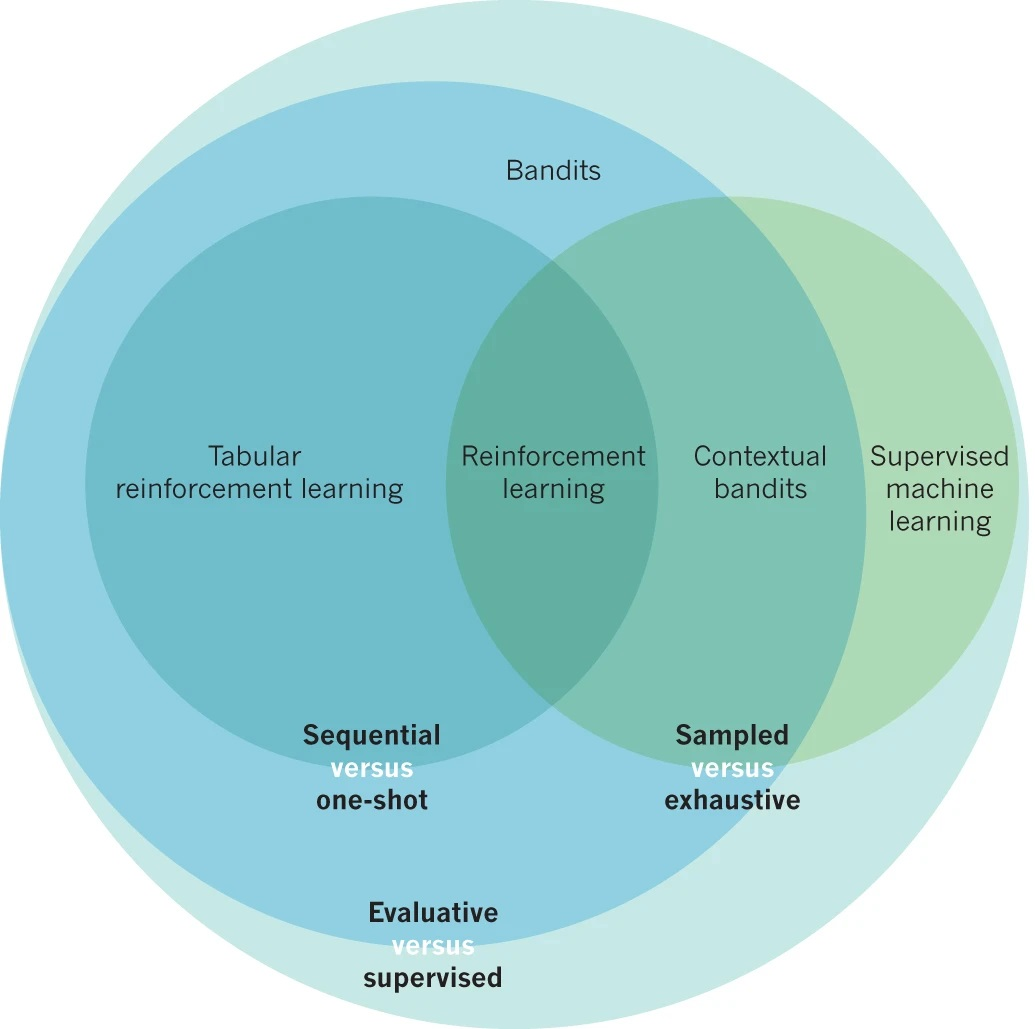
\includegraphics[width=0.35\textwidth]{diff.jpg}
    \caption{Decisions of machine-learning feedback \cite{littman2015reinforcement}}
    \label{fig:learning_prob}
\end{figure}

The first dimension we examine is whether the learner is exposed to all possible situations. Consider the difference between plain memorization and supervised learning. In the first case, all valid key-solution pairs are presented to the system during training, whereas in the latter case, the training set is merely a sampled subset of all possible situations, and the learner is expected to perform on instances that may never appear during training. 

Another example is the difference between Tabular RL and Approximate RL. In tabular RL, because the state and action spaces are small enough for the value functions to be represented in arrays, convergence to optimum is often guaranteed, provided enough occasions of traversals. On the other hand, in approximate RL, the state space's size is either infinite or beyond computational limits. As such, the majority of potential states are not to be examined in training, and those in the training set are not likely to reappear during testing. Hence, in this case, we need to focus on generalization: to utilize feedback from a limited subset of the state space for applications on a broader subset \cite{sutton_reinforcement_1998}.

Mathematically speaking, in Exhaustive problems the learner is given all valid combinations of the states and labels: 
\begin{equation}
    D_{train}=\{(s,a)\,|\,\forall s\in \mathcal{S}, \forall a \in \mathcal{A}, (s,a) \;\mathrm{valid}\}, D_{test} \subseteq D_{train}
\end{equation}
In Sampled feedback problems, the learner is only allowed access to samples drawn from the true distribution:
\begin{equation}
    D_{train}=\{(s_i,a_i)\,|\,s_i,a_i\sim \mathcal{D}(s,a),i=1,...,N\}, 
    D_{test}\nsubseteq D_{train}
\end{equation}

The second dimension is whether we have information for all possible actions (labels) given an arbitrary state. If so, the feedback is said to be instructive (supervised), as opposed to evaluative feedback. In supervised learning, we have a ground truth label for each encountered state. This is equivalent to having a Boolean mask (which yields true only at Ground Truth) on the action (label) space for each state:
\begin{equation}
    \forall (s_i,a_i)\in D_{train}, \forall a\in \mathcal{A}(s_i): \mathrm{Receive \;Mask}[s_i,a]=(a==a_i)
\end{equation}
The instructive mask here presents which $a\in A(s)$ is the best.

On the other hand, in RL we rely on either the reward received from executing the current action, or the return (cumulative rewards) corresponding to a sequence of state-actions. At each step, we have at most an numerical value only for the action executed, which is insufficient to determine whether this specific action is the best among the action space.
\begin{equation}
    \begin{matrix*}
    \forall (s_i,a_i)\in D_{train}: \mathrm{Receive\;} R(s_i,a_i) \sim P(r\;|\;s_i,a_i) \;\;\;\; (\mathrm{No}\;R(s_i,\forall a\in A(s_i))\\
    \mathrm{or}\\
    \forall \zeta_i \in D_{train}: \mathrm{Receive\;} G(\zeta_i) \sim P(g\;|\;\zeta_i) \;\; \mathrm{where} \;\; \zeta_i = \{(s_t,a_t)\}_{iT+1:(i+1)T}\;\;\;\; (\mathrm{No}\;G(\forall \zeta)\\
    \end{matrix*}
\end{equation}
In either case, the reward (or return) only presents how well the action (or sequence) is, but not whether it is the best or the worst. Such a phenomenon demands exploration in search of better actions \cite{sutton_reinforcement_1998}.

The third dimension is whether the outcome of action affects the next state. Consider a problem where the learner repeatedly faces k different actions. After choosing an action, the learner receives a reward that follows a probability distribution conditional to the action. If the probability $R(a)$ is fixed, the problem is called the k-arm bandit. If the probability is non-stationary, i.e., $R\sim R(s,a)$ but $S\indep A$, the problem is called contextual k-arm bandit. Either way, the environment (and the state drawn) must be independent of the actions.

The characteristic described above is called one-shot. On the other hand, the sequential case refers to when states are indeed affected by previous actions. In this case, we need to learn not only the reward distribution $R(s,a)$, but also the system dynamics $P(s'\;|\;s,\,a)$ \cite{sutton_reinforcement_1998}.

\section{Summary}

\subsection{Online Learning}
\normalfont
Online learning algorithms are primarily used to tackle predictive or sequential decision-making tasks that require learning from a continuous stream of data instances. The pseudo-code for the family of online learning algorithms is summarized in Algorithm \ref{algo:wma} below. The update equations on line 7 and 8 state that $\theta$ is updated based on how similar the learner's predictions are to the target distribution.

\begin{algorithm}[H]
\caption{Online Learning}
\label{algo:wma}
\begin{algorithmic}[1]
\STATE Initialize Nature \hfill $\triangleright$ black box model that emulates the target distribution
\STATE Initialize the parameters ($\theta$) of the Online Learner
\FOR{$trial=1,\;\cdots,\;\text{Number of Trials}$}
    \FOR{$t=1,\;\cdots,\;\text{Sequence Length}$}
    \STATE $x^{(t)}, y^{(t)}\leftarrow$ \textsc{Sample Nature} ($t$) \hfill $\triangleright$ Obtain the target input-output pair
    \STATE $\hat{y}^{(t)}\leftarrow$ \textsc{Online Learner} ($x^{(t)} | \theta$) \hfill $\triangleright$ Estimate the output conditioned on the $x^{(t)}$ and $\theta$
    \STATE $l\leftarrow$ \textsc{Loss Function} ($y^{(t)}, \hat{y}^{(t)}$) \hfill $\triangleright$ Calculate the loss of the model
    \STATE $\theta \leftarrow$ \textsc{Update parameters} ($ l, \theta$) \hfill $\triangleright$ Update the online learner\ENDFOR
\ENDFOR

\end{algorithmic}
\end{algorithm}

The family of online learning algorithms share the following properties:
\begin{itemize}
  \item The algorithm must make predictions and learn on-the-fly
  \item Sequence streams are assumed to be uncorrelated
  \item Require immediate feedback in terms of a loss or a reward conditioned on the recent prediction
  \item Requires access to the entire state or the sampled state
\end{itemize}

Moving ahead, the domain of online learning encompasses algorithms such as Predictions with Expert Advice \cite{vovk1998game}, Bandits\cite{whittle1980multi}, and Contextual Bandits \cite{lu2010contextual}, which all attempt to minimize the loss of the model's prediction against the known reference provided by the Environment. We can formally interpret this as an optimization problem that addresses the following cumulative loss:
\begin{align}
  \underset{\hat{y}}{argmin} = \sum_{t=1}^T l(y^{(t)}, \hat{y}^{(t)} )
\end{align}

\subsection{Online Learning vs. Supervised Learning}
\normalfont
Online learning differs from supervised learning mainly in terms of the ability of the model to access data. In a supervised setting \cite{super}, the algorithm attempts to approximate a stationary data-distribution, and usually involves a training and testing regime. Whereas in the online setting there is no specific training or testing datasets or stages. The online learning algorithms usually involve incrementally learning the distribution using the sequences of input and output pairs. Due to the nature of the data collection procedure, online learning algorithms tend to be more agile, and can adapt quickly to shifts in the data-distribution, which can be stochastic, deterministic, or adversarial. Thus, online learning algorithms prove to be the preferred choice for robotic learning algorithms. 

As both supervised learning algorithms, and online learning algorithms, learn models that map a given input space to a desired approximation of the output distribution, selecting the appropriate algorithm boils down to identifying the appropriate characteristics that define the problem at hand. The main design choices that need to be considered when deciding between supervised and online learning algorithms are:
\begin{itemize}
  \item Is the data distribution changing over time?
  \item Is the evaluative or instructive feedback incremental?
  \item Is the training dataset too large to process all at once?
\end{itemize}

\subsection{Prediction With Expert Advice (PWEA)}
\normalfont
To motivate the use of PWEA, we will present a learning problem involving gamblers and racehorses. In this motivating example, we have a set of expert gamblers who routinely bet on horses. As an outsider, we intend on identifying the best expert from the set of experts and mimic their bets. We start by weighing all the experts equally. Next, we update our weights based on the accuracy of each expert. We penalize the experts who incorrectly predicted the outcome of the horse race, by reducing their share of weights to zero. Then, we reinitialize our distribution of weights by equally distributing the weights among experts who correctly predicted the outcome of the race. This process is repeated iteratively until we converge to the subset of the best experts.

The pseudo-code for the PWEA algorithm is summarized in Algorithm \ref{algo:pwea} below. The update equations on line 8 state that the set $E$ is updated based on the performance of each expert. Experts that perform poorly are removed from the set, and experts that succeed, remain in the set under consideration. The performance is evaluated by an external black-box entity, represented as Nature in Algorithm \ref{algo:pwea}. 

\begin{algorithm}[H]
\caption{Predictions With Expert Advice}
\label{algo:pwea}
\begin{algorithmic}[1]
\STATE Initialize the set of experts $E$ \hfill $\triangleright$ these are similar to classes
\STATE Initialize Nature \hfill $\triangleright$ black box model that evaluates each expert
\FOR{$trial=1,\;\cdots,\;\text{Number of trials}$}
    \STATE $y_{E}^{(t)}\leftarrow$ \textsc{Sample Nature} ($t$) \hfill $\triangleright$ Evaluate the performance
    \STATE $E\leftarrow \{e | y_{e} = \text{success}\} $ \hfill $\triangleright$ Update E conditioned on the performance of each expert
\ENDFOR

\end{algorithmic}
\end{algorithm}

PWEA has the characteristics of an online learning algorithm. It is suitable for data streams that are one-shot in nature. This ascertains that the individual data streams are uncorrelated and do not affect each other. Thus, the order of the dropping of the experts is independent with respect to the final convergence of the algorithm. Thus, the final result is independent of the stochastic ordering of the streams. PWEA is also instructive in terms of the feedback provided to the learning algorithm. Thus, the online learner receives the fully observable loss based on its predictions. This translates to obtaining the complete information required to evaluate if the expert was indeed right or wrong. The notion of experts in the PWEA framework can be mapped to classes in the supervised learning setting. Finally, the PWEA algorithm is exhaustive in nature, as we have access to the entire action space, which is finite in size. Thus, it is theoretically possible to exhaustively search the action space. However, it should be noted that the action space is exponential with respect to the number of experts.

\subsection{Greedy/Consistent Algorithm}
\normalfont
The Consistent (Greedy) Algorithm is similar to the PWEA mentioned in the last section; however, the expert selection is slightly modified. The Consistent algorithm does not maintain a set, like the PWEA. Instead, the algorithm maintains a stack, and pop's experts from the stack based on their performance. The algorithm will converge once the best expert has been encountered. It should be noted that the greedy algorithm need not investigate every expert nor empty the stack to converge upon the best expert. Assuming a \textit{best expert} exists, then it will take a maximum of $N$ trials to identify the expert, where $N$ is the number of experts. One drawback of this method is that it can only identify at the most one expert. Thus, if the set of \textit{best experts} comprises of more than one element, this method will fail to identify all experts in the desired set.

Before formally presenting the greedy algorithm, we will introduce the notation required to mathematically ground the algorithm. We define the instance domain $\chi$ as the set of all possible outcomes. Intuitively, this can be thought of as the set of all possible \textit{advice} expressed by each expert. We denote the advice of all the experts at a given timestamp $t$, as a vector $x^{(t)}$, which has the dimensionality based on the size of the number of experts. Next, we define the target domain $\mathcal{Y}$, which is the space of all outcome values for each expert. We denote the outcome of all the experts at a given timestamp $t$, as a vector $y^{(t)}$, which has the dimensionality based on the size of the number of experts. Finally, we define the hypothesis class $\mathcal{H}$, as the set of all selector or indicator functions. Intuitively, this can be thought of as a way to poll a given expert. We can write the relationship between vectors in these three spaces as follows:
\begin{align}
  \hat{y} = h_e(x)=x_e
\end{align}

We summarize the notation below:
\begin{itemize}
    \item $x^{(t)} \in \chi \subset \mathcal{R^E}$
    \begin{itemize}
      \item $\chi$ is the instance domain
      \item $x^{(t)}$ is an E-dimensional vector of expert advice
      \item $x_e^{(t)}$ is the advice of the expert $e$ at trial t
    \end{itemize}
    \item $y^{(t)} \in \mathcal{Y} =\{0,1\}$
    \begin{itemize}
      \item $\mathcal{Y}$ is the target domain
      \item $y^{(t)}$ is the outcome of expert $e$ at trial t
    \end{itemize}
    \item $h \in \mathcal{H} =\{h_1,...h_E\}$
    \begin{itemize}
      \item $\mathcal{H}$ is the hypothesis class
      \item $h$ is the expert selector function
      \item $h_e$ is a function that is defined as $\hat{y} = h_e(x)=x_e$
    \end{itemize}
\end{itemize}

The pseudo-code for the greedy algorithm is summarized in Algorithm \ref{algo:greedy} below. The update equations on line 7 state that the version space $V^{(t)}$ is updated based on the performance of each expert. Experts that perform poorly are removed, and experts that succeed, remain under consideration.

\begin{algorithm}[H]
\caption{Greedy Algorithm}
\label{algo:greedy}
\begin{algorithmic}[1]
\STATE Initialize $V^{(1)} = \mathcal{H}$ \hfill $\triangleright$ Initialize the version space to store all hypothesis
\FOR{$t=1,\;\cdots,\;\text{Number of Trials}$}
    \STATE \textsc{Receive}$(x^{(t)})$ \hfill $\triangleright$ Obtain the expert advice
    \STATE $h=$\textsc{FirstElement}$(V^{(t)})$  \hfill $\triangleright$ Greedy selection \& prediction (pop from stack)
    \STATE $\hat{y}^{(t)}=h(x^{(t)})$
    \STATE \textsc{Receive}$(y^{(t)})$ \hfill $\triangleright$ Obtain true outcome
    \STATE $V^{(t+1)}=\{h \in V^{(t)} : h(x^{(t)})= y^{(t)}\}$  \hfill $\triangleright$ Update the consistent hypothesis
\ENDFOR

\end{algorithmic}
\end{algorithm}

The greedy algorithm delineated in Algorithm \ref{algo:greedy}, details the process of obtaining the best expert. Initially, we initialize the version space to the whole hypothesis space. This can be justified as we don't know which hypothesis is correct, and thus intermittently hold the belief that all possible hypotheses are potential solutions. Next, we iterate over the different trails, and first receive the different expert advice by polling our experts. Next, we select the first expert based on the initialization of the stack. As the algorithm is greedy, we are only concerned with the element on the top of the stack. Next, we use this selection function to obtain our estimate for the outcome. Finally, we obtain our true outcome, and update our version space using the newly acquired information. This update is performed by only retaining the set of hypotheses that are in agreement with our most recent outcome. 

The greedy algorithm has a fair set of assumptions, specifically in terms of realizability \cite{ohta1984reachability}. We assume that there exists a hypothesis $h^*$ that maps $\chi \to \mathcal{Y}$.

It is worthwhile noting that the consistent algorithm makes mistakes before identifying the perfect hypothesis. As demonstrated in Fig \ref{fig:loss}, these mistakes would result in a loss compared to the case where we knew the perfect hypothesis in hindsight. In the next section, the upper bound of the number of such mistakes is discussed.

\begin{figure}
    \centering
    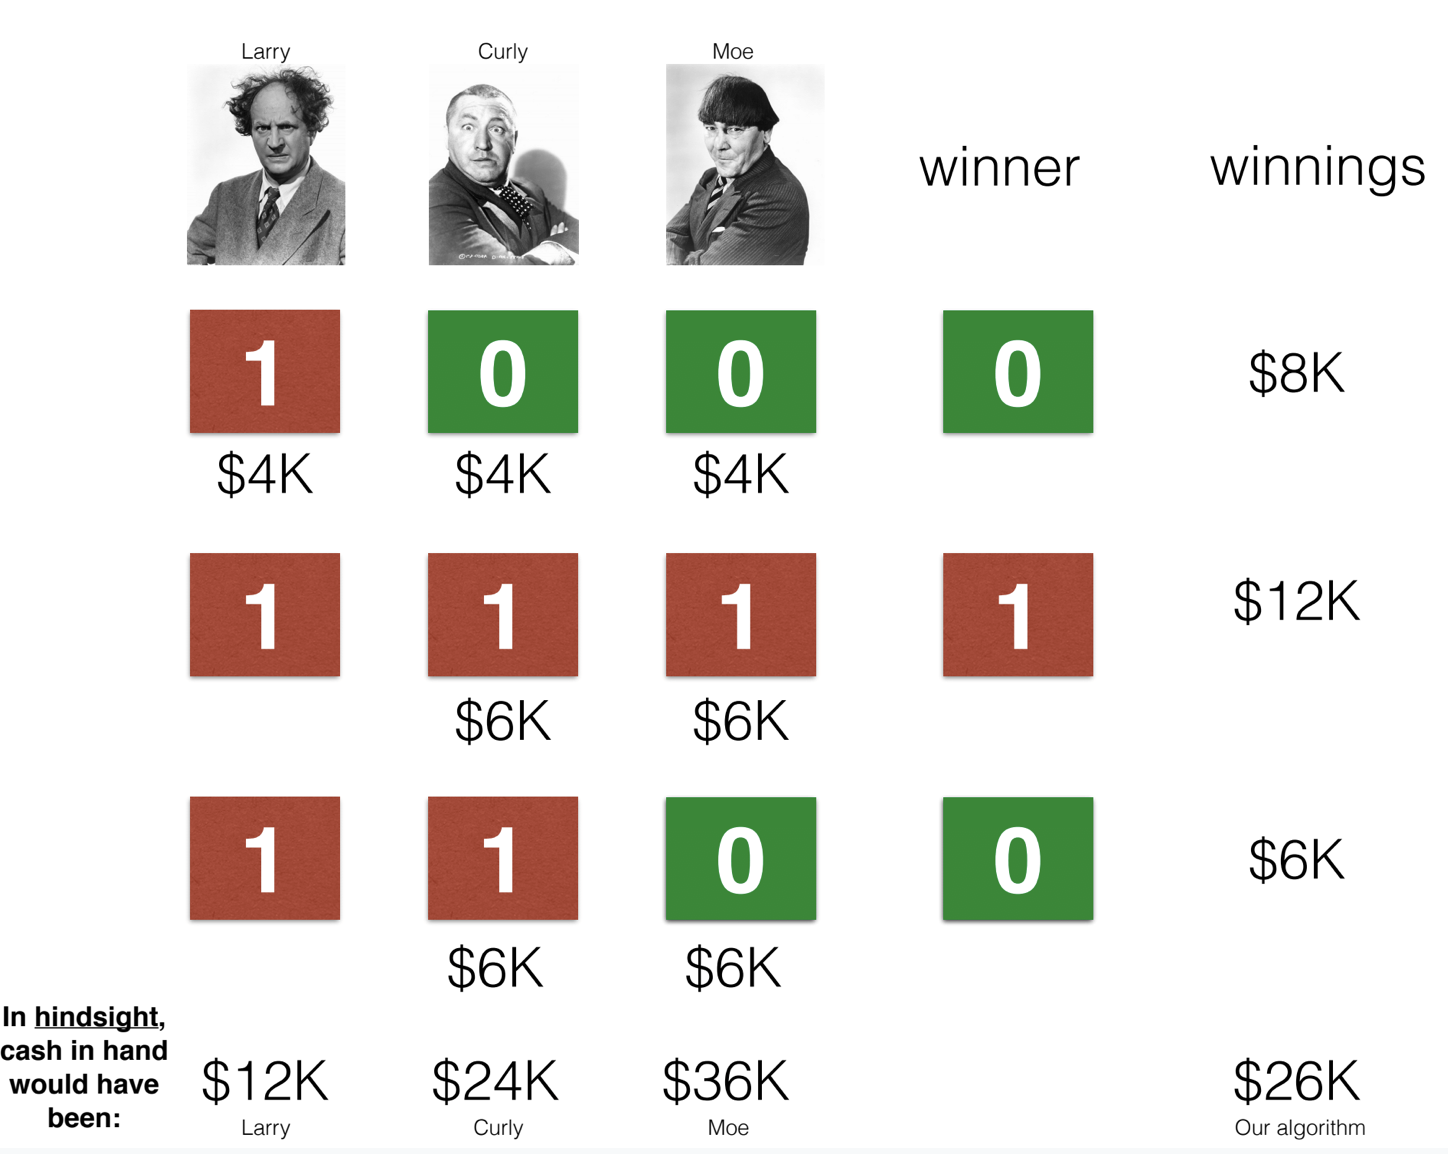
\includegraphics[width=0.5\textwidth]{fig2.png}
    \caption{Loss in Winnings}
    \label{fig:loss}
\end{figure}



\subsection{Analysis of the Consistent Algorithm}

Assume realizability (the perfect hypothesis is in the hypothesis class); it is known that the version space will converge to the set only containing perfect hypotheses, after enough mistakes are made. The question is, is there an upper bound for the number of mistakes the algorithm could make, before it eliminates all imperfect hypotheses? 

\begin{theorem}
Let $p^{(t)}\in\{1,0\}$ denote whether the consistent algorithm makes a mistake at an arbitrary timestamp $t$. Let $M_c(\mathcal{H})\doteq\sum_{\tau=0}^{t-1}p^{(\tau)}$ represent the total number of mistakes made by the algorithm. Then, $M_c(\mathcal{H})\leq |\mathcal{H}|-1$.
\end{theorem}

\begin{proof}
At any timestamp $\tau$, the following relationship holds true:
\begin{equation}
    |V^{(\tau)}|\leq|V^{(\tau-1)}|-p^{(\tau-1)}
    \label{eqn:iter}
\end{equation}
because the algorithm removes at least one (the first) hypothesis from the version space after a mistake was made.

Taking the summation on both sides of the equation \ref{eqn:iter} from timestamp $\tau=1$ to any $t$ yields:
\begin{equation}
    \forall t:\sum_{\tau=1}^t|V^{(\tau)}|\leq \sum_{\tau=0}^{t-1}|V^{(\tau)}|-\sum_{\tau=0}^{t-1}p^{(\tau)}
    \label{eqn:summation}
\end{equation}

With basic algebra, equation \ref{eqn:summation} evaluates to:
\begin{equation}
    \forall t:|V^{(t)}|\leq |V^{(0)}|-\sum_{\tau=0}^{t-1}p^{(\tau)}=|\mathcal{H}|-\sum_{\tau=0}^{t-1}p^{(\tau)}
    \label{eq:ana1}
\end{equation}
Note that the initial version space is identical to the entire hypothesis space $\mathcal{H}$.

Under the assumption of realizability, it is guaranteed that the version space always contains a perfect hypothesis:
\begin{equation}
    \forall t: |V^{(t)}|\geq 1
    \label{eq:ana2}
\end{equation}

Combining equation \ref{eq:ana1} and \ref{eq:ana2}, we bound the size of the version space:
\begin{equation}
    \forall t: 1\leq|V^{(t)}|\leq |\mathcal{H}|-\sum_{\tau=0}^{t-1}p^{(\tau)}
\end{equation}
Substitute in the notation of $M_c(\mathcal{H})$, the upper bound of total mistakes made by the consistent algorithm is:
\begin{equation}
    M_c(\mathcal{H})\leq |\mathcal{H}|-1
\end{equation}
\end{proof}



From the derivation above, we conclude the common strategy for bound derivations.
\begin{itemize}
    \item Define 'potential' function (the size of the version space $|V|$).
    \item Upper bound the potential function.
    \item Lower bound the potential functions.
    \item Combine the bounds.
    \item Use algebra or approximation to get the performance bound.
\end{itemize}

It is worth mentioning that online learning theory focuses on the theoretical bounds of algorithm performance. Such guarantees are often vital to the reliability demands in robotic systems.

\bibliography{refs}
\bibliographystyle{abbrv}

\newpage
\section{Appendix}

We found an image that helps illustrate weighting in a general PWEA:
\begin{figure}[ht]
    \centering
    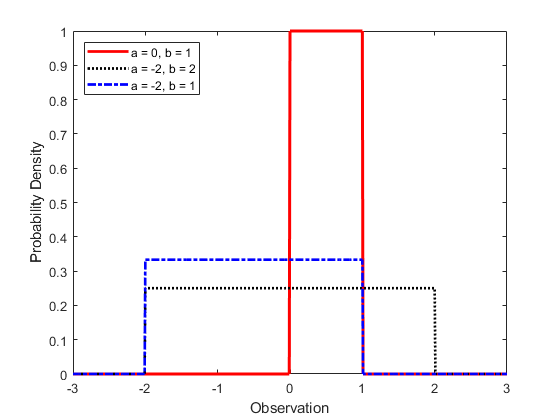
\includegraphics[width=0.5\textwidth]{ContinuousUniformDistributionPdfExample_01.png}
    \caption{Weighting in PWEA.}
    \label{fig:weighting}
\end{figure}

Figure \ref{fig:weighting} above shows the iterative concentration of weights by removing under-performing experts. We start with the dotted black distribution, re-weight our belief to obtain the dotted blue distribution, and finally re-weight again to converge on the red distribution. The red distribution illustrates the convergence and identification of the best expert from the set of experts.

\end{document}


